在实现各种功能的过程中,总会发现一块开发板的引脚不够用的情况,此时我考虑使用多块开发板进行开发。
除使用I2C、SPI、UART等协议进行开发板之间的通信之外,本身支持Wifi的ESP32中还有一个由乐鑫公司开发的协议ESP-NOW,
可以无线(即占用更少的引脚)实现两块ESP之间的通信。

我使用ESP32作为主控,主控中调配语音识别大模型,ESP8266中作为从控,调用各种传感器,如DHT11湿温度模块。

通过ESP-NOW协议实现两块ESP之间的通信,读取从控中获取的参数。根据官方手册中的Examples:\href{https://docs.espressif.com/projects/arduino-esp32/en/latest/api/espnow.html?highlight=esp\%20now}{\underline{ESP-NOW.html}},我仿照其代码成功实现了通信。

\subsubsection{获取主板唯一MAC地址}

\begin{lstlisting} [language = C++, title = {获取主板唯一MAC地址}]
    void setup() {
        Serial.begin(115200); // 每一块板的MAC地址是唯一的
        WiFi.mode(WIFI_MODE_STA); // 知道MAC地址后就可以向主机发送信息
        Serial.println(WiFi.macAddress());
    }
\end{lstlisting}

通过上传代码,我将我所需开发板的MAC地址记录在此:

\begin{itemize}
    \item 主板:BC:DD:C2:D0:07:B4
    \item 从控(32):1C:69:20:2B:9D:58
    \item 从控(32E):EC:64:C9:90:6B:74
    \item 从控(32 Side):BC:DD:C2:CD:07:00
    \item 从控(8266):待使用
\end{itemize}

\subsubsection{扫描I2C设备地址}

需要使用IIC协议通信的传感器(如MPU6050),必须需要设备的IIC地址(如\texttt{MPU.begin(0x68,\&Wire);})
使用Wire.h库中的接口扫描,得到 $0x68$。I2C接口不止可以插一根,根据不同的通信地址可以在同一个引脚处插入多个IIC通信。

\begin{lstlisting} [language = C++, title = {扫描I2C设备地址}]
    Wire.begin();  // 初始化I2C总线
    Serial.begin(115200);

    // 扫描所有可能的I2C地址
    for (uint8_t address = 1; address < 127; address++) {
        Wire.beginTransmission(address);
        uint8_t error = Wire.endTransmission();

        if (error == 0) {
            Serial.print("I2C device found at address 0x");
            if (address < 16) Serial.print("0");
            Serial.print(address, HEX);
        }
    }
\end{lstlisting}

\subsubsection{主机(Master)、从控(Slave)代码}

主机(Master)代码:

在根据Examples的运作时,我的ESP-NOW发送数据一直是失败的,
查阅资料后发现要加入一行代码:

\texttt{peerInfo.ifidx = WIFI\_IF\_STA;}

暂不理解为什么其他示例没有这行代码也可以运行,
参考资料:\href{https://esp32.com/viewtopic.php?p=132946}{\underline{https://esp32.com/viewtopic.php?p=132946}}。

\begin{lstlisting} [language = C++, title = {主机(Master)代码}]
// 定义接收到的数据结构
typedef struct struct_message {
    float accelX;
    float accelY;
    float accelZ;
    float temperature;
} struct_message;

struct_message incomingData;

void onDataRecv(const uint8_t * mac, const uint8_t *data, int len) {
    // 将接收到的字节数据解释为结构体类型
    struct_message *receivedData = (struct_message *)data;
}

void setup {
    WiFi.mode(WIFI_STA); // 设置为站点模式
    // 设置对等设备信息
    esp_now_peer_info_t peerInfo;
    peerInfo.channel = 0;
    peerInfo.encrypt = false;
    peerInfo.ifidx = WIFI_IF_STA; // 注意!此步骤一定要有
    // 注册接收回调函数
    esp_now_register_recv_cb(onDataRecv);
}

\end{lstlisting}

从机关键代码,其余部分与主机相似:

\begin{lstlisting} [language = C++, title = {从机(Slave)代码}]
// 目标主机的MAC地址(需要替换为实际的主机MAC地址)
uint8_t masterMACAddress[] = {0xBC,0xDD,0xC2,0xD0,0x07,0xB4};

// 发送回调函数
void onDataSent(const uint8_t *mac_addr, esp_now_send_status_t status) {
    Serial.print("Last Packet Send Status: ");
    Serial.println(status == ESP_NOW_SEND_SUCCESS ? "Delivery Success" : "Delivery Fail");
}

void loop {
    esp_err_t result = esp_now_send(masterMACAddress, (uint8_t *)&myData, sizeof(myData));
}
\end{lstlisting}

\subsubsection{数据传输的关键步骤}

由于在数据传输时,在主机(Master)处只注册了一个回调函数,但从机(Slave)发送的数据有很多种(我定义了不同的结构体来存储变量),
考虑到可能出现结构体对齐问题,不妨将各部分结构体多定义出一个变量,使得接收时可以先判断这个结构体的大小以判断接收到的是什么传感器的数据,接下来再进行数据解析。

\begin{lstlisting} [language = C++, title = {主机读取结构体大小以判断数据来源}]
// 8 字节                          // 12 字节                           // 16 字节
typedef struct DHT22Message {     typedef struct MPU6050Message {       typedef struct MQ5Message {
    float temperature;                float UpAndDown;                      float h2PPM;
    float humidity;                   float LeftAndRight;                   float ch4PPM;
} DHT22Message;                       float temperature;                    float lpgPPM;
                                  } MPU6050Message;                         float flagMQ5;
.......                                                                 } MQ5Message;
\end{lstlisting}

\begin{figure}[H]
    \centering
    \begin{subfigure}[b]{0.42\textwidth}
        \centering
        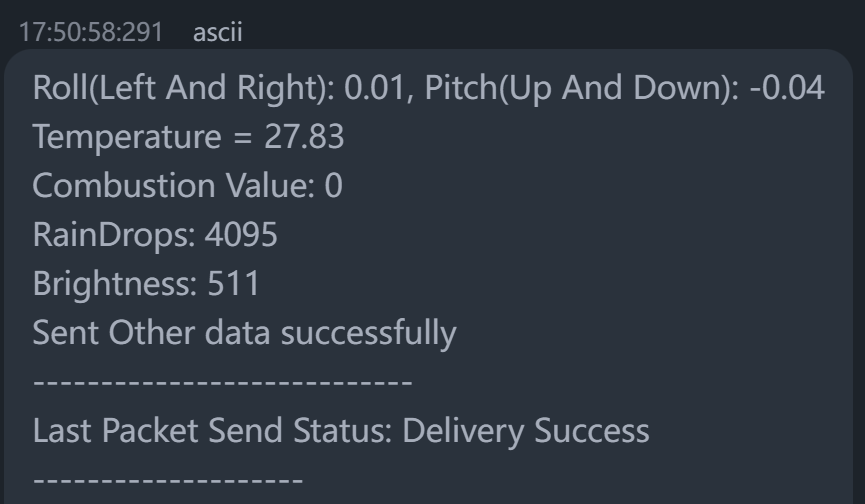
\includegraphics[width=\textwidth]{img/ESP32-Slave-SendData.png}
        \caption{从机发送数据}
        \label{fig:DHT22_active}
    \end{subfigure}
    \hspace{4em}
    \begin{subfigure}[b]{0.325\textwidth}
        \centering
        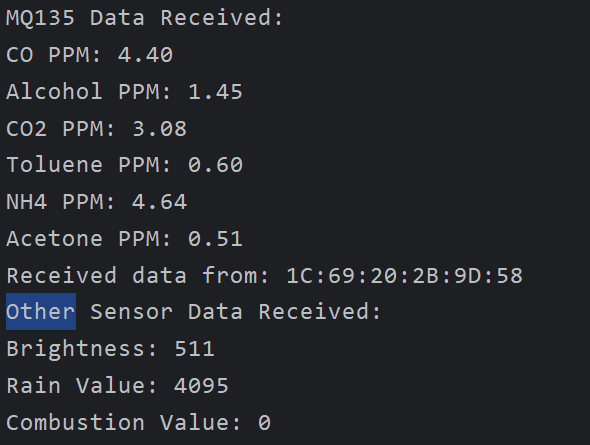
\includegraphics[width=\textwidth]{img/ESP-Master-ReceivedData.png}
        \caption{主机读取数据}
        \label{fig:MPU6050_active}
    \end{subfigure}
    \caption{基于ESP-NOW的数据传输成功}
    \label{fig:combined}
\end{figure}

\subsubsection{ESP与Wifi建立通信}

首先,进入TP-Link路由器的管理界面,室内路由器使用Mesh组网,故使用默认配置地址192.168.0.1。

注意,ESP系列硬件仅支持2.4GHz的无线网络通信,故开启2.4GHz的Wifi。

\begin{figure} [H]
    \centering
    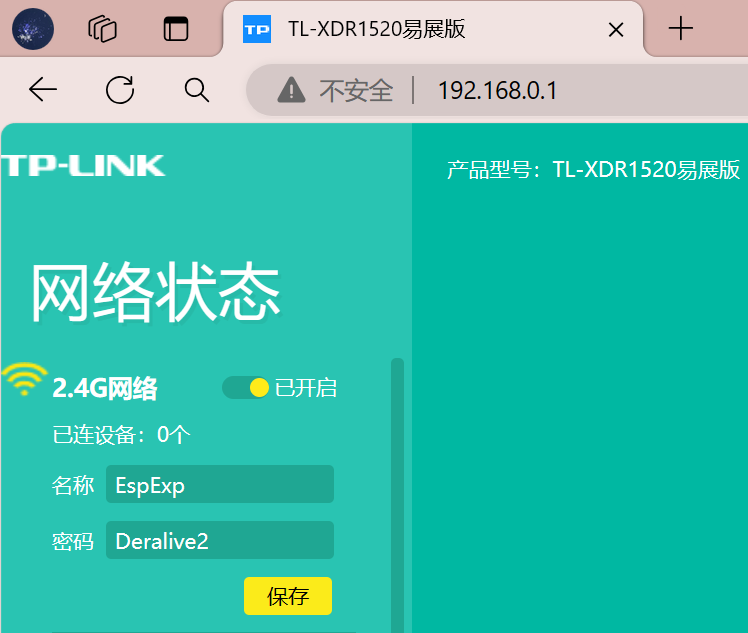
\includegraphics[width=0.3\textwidth]{../img/Wifiset.png}
    \caption{TP-Link路由器管理界面}
\end{figure}

通过Wifi.h库中的接口,进入WifiSTA.cpp查看所有接口(见附件-1),使用Wifi.begin()函数连接到路由器。

\begin{figure} [H]
    \centering
    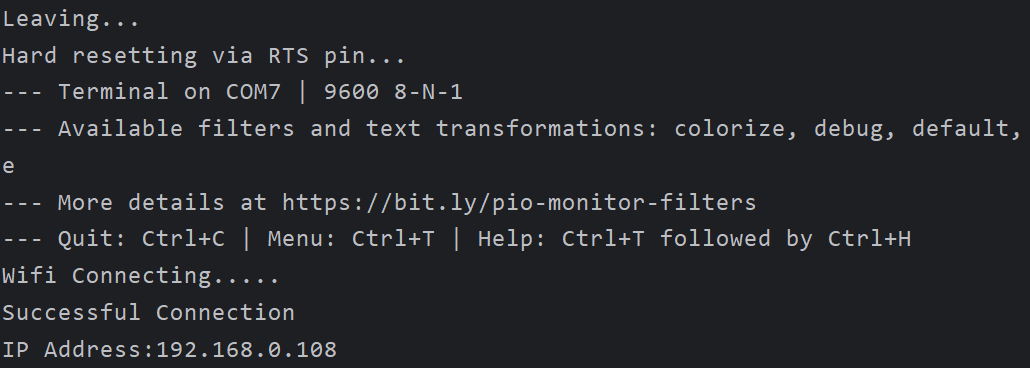
\includegraphics[width=0.5\textwidth]{../img/WifiConnectingSuccess.png}
    \caption{ESP32与Wifi成功建立连接}
\end{figure}

\subsubsection{发送HTTP请求}

心知天气提供免费的天气API查询接口:\href{https://www.seniverse.com/}{https://www.seniverse.com/},先用此进行测试,后续可调用更多API。

\begin{figure} [H]
    \centering
    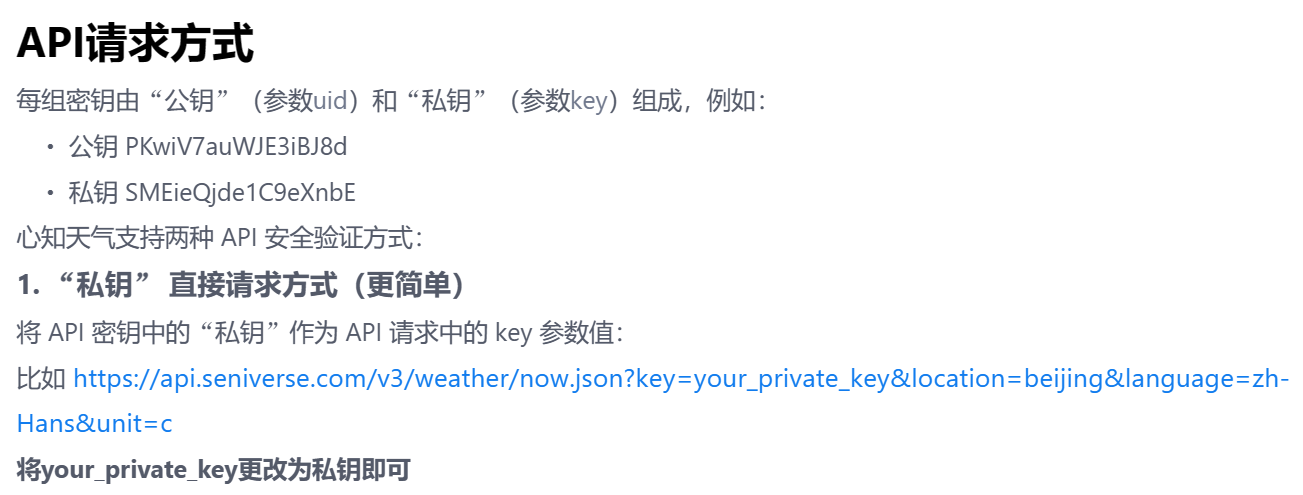
\includegraphics[width=0.5\textwidth]{../img/WeatherAPI.png}
    \caption{心知天气API}
\end{figure}

使用HTTPClient.h库,向服务器发送HTTP请求,并接收服务器的响应。使用代码如下所示:

\begin{lstlisting}[language = C++, title = {发送HTTP请求并解析JSON数据}]
  // 创建 HTTPClient 对象并发送 Get 请求
  HTTPClient http;
  http.begin(url+"?key="+key+"&location="+city+"&language="+language+"&unit="+unit);
  int httpCode = http.GET();

  // 获取响应状态码及正文
  Serial.printf("HTTP Status Code: %d", httpCode);
  Serial.print("\n");

  String response = http.getString();
  Serial.println("Response Data:");
  Serial.println(response);

  http.end();

  // 解析 JSON 数据
  DynamicJsonDocument doc(1024);
  deserializeJson(doc, response);

  // 从解析后的 JSON 文档中获取值
  unsigned int temp = doc["results"][0]["now"]["temperature"].as<unsigned int>();
  String info = doc["results"][0]["now"]["text"].as<String>();

  Serial.printf("Daytime temperature: %d\n", temp);
  Serial.printf("Daytime Weather: %s\n", info);
\end{lstlisting}

上传并监视,使用VOFA+ 1.3.10,通信成功,数据解析成功,结果如下图所示:

\begin{figure} [H]
    \centering
    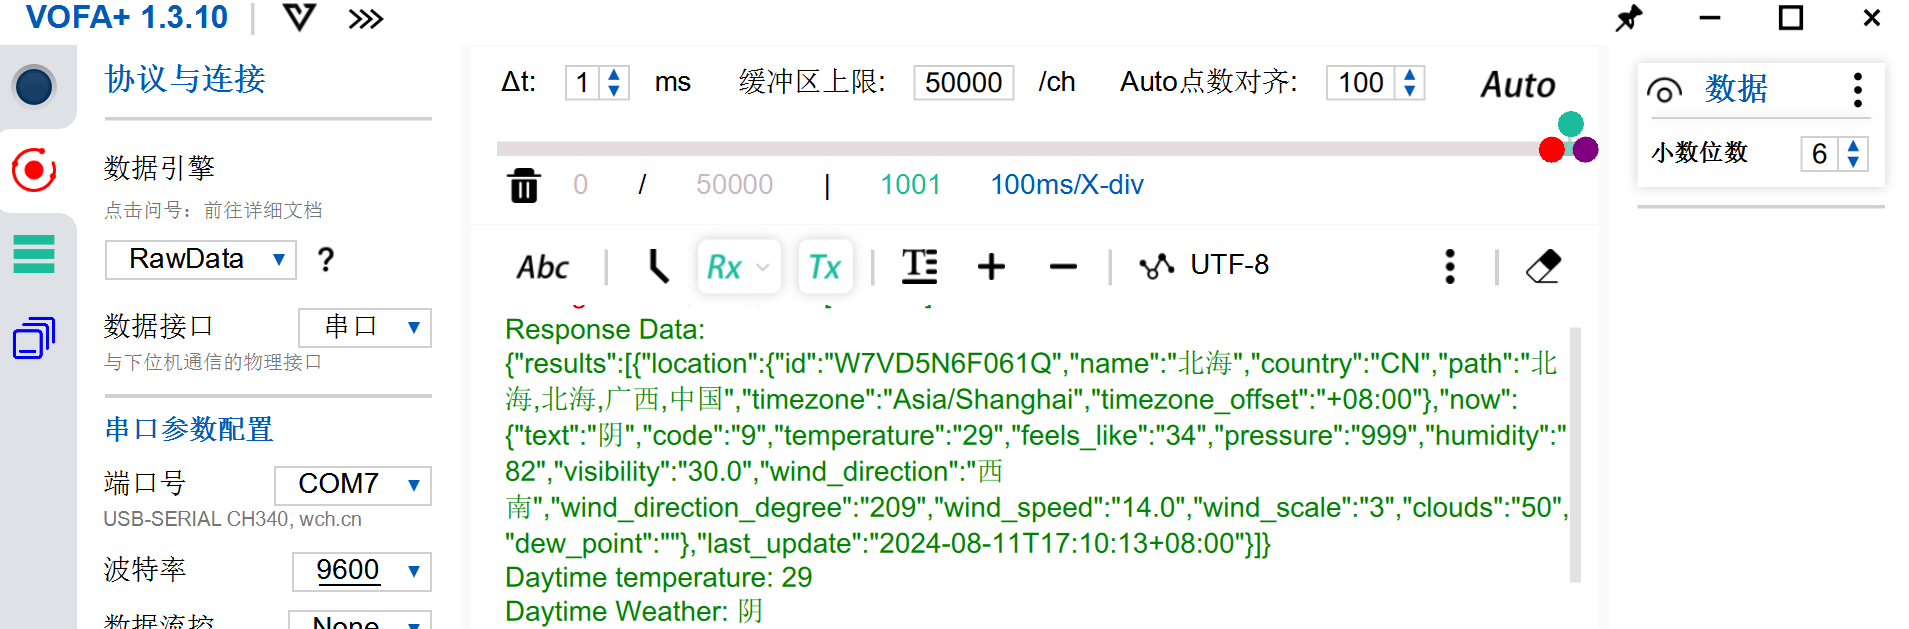
\includegraphics[width=0.7\textwidth]{../img/SerialWeatherInformation.png}
    \caption{天气数据}
\end{figure}